\chapter{Introduction}
\todo{this is a todo eample.}
\liwen{this is a commnet example.}


We consider the problem of merging two arrays $A$ and $B$ into a single array $C$. 
Each element in the array has a key. An ordering relation denoted by $\leq$ 
is defined on the keys. Array $A$ and $B$ has $m$ and $n$ elements, respectively, where 
$m$ and $n$ do not have be to equal.  
Both array $A$ and array $B$ are sorted based on the ordering relation. 
The task is to produce the output array $C$ of size $m+n$.  
Array $C$ consists of all the input elements from array $A$ and $B$, and is 
sorted by the ordering relation. 

Figure \ref{fig:merge} gives an example of merging two arrays of integers.  
\begin{figure}[!th]
\begin{center}
\resizebox{\textwidth}{!}{
    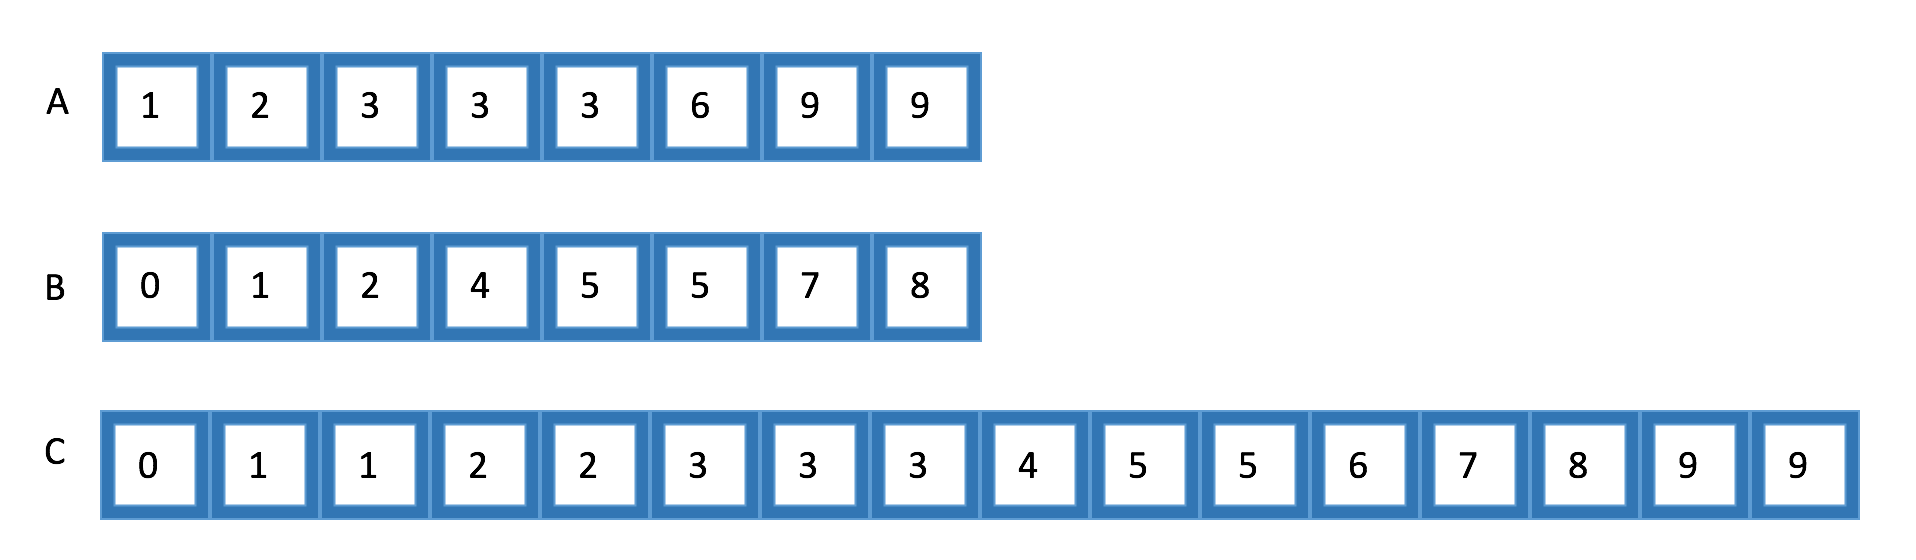
\includegraphics{merge.png}
}
\end{center}
\caption{{\label{fig:merge}} Merge Example}
\end{figure}

Sequentially merging two sorted arrays has been solved for a long time. Listing 
\ref{list:merge_origin} shows the sequential code implemented in C++.  
The time complexity of this implementation is $O(m+n)$. 

        \begin{minipage}{\linewidth}
        \begin{singlespace}
        \begin{lstlisting} [caption = {Sequential Merge Implementation in C++}, captionpos=b, label = {list:merge_origin}]
void merge(int *A, int m, int *B, int n, int *C) 
{
    int i, j, k, l;
    i = 0;              //index A
    j = 0;              //index B
    k = 0;              //index C
  
    /* handle the start of A[] and B[] */
    while ((i < m) && (j < n))
    {
        if (A[i] <= B[j]) {
            C[k] = A[i];
            i++;
        } else {
            C[k] = B[j];
            j++;
        }
        k++;
    }
    if (i == m) {       //handle remaining b[]
        for (l = j; l < n; l++) 
        {
            C[k] = B[l];
            k++;
        }
    } else {            //handle remaining a[]
        for (l = i; l <m; l++) 
        {
            C[k] = A[l];
            k++;
        }
    }
}
        \end{lstlisting}
        \end{singlespace}
        \end{minipage}


Merge is an important operation in contemporary computing systems. It is used as a subroutine
by many popular algorithms and applications such as merge sort 
and database operations. Therefore, the performance of merging is critical. 

As single-chip multiprocessors (CMPs) become more and more popular, parallel merging algorithms are 
developed to exploit the performance of CMPs. 
In \cite{pmalgo}, Siebert et al. proposed a parallel merge algorithm. 
With $p$ processing elements, 
the time complexity of merge could be reduced from $O(m+n)$ to $O(\frac{m+n}{p} + \log min(m,n))$.
This parallel merge algorithm can be implemented on CMPs using openMP with minimum effort, 
and achieve considerable speedup compared to
the sequential merge. 

However, a direct implementation of this parallel merge algorithm on GPU will result in 
suboptimal performance due to the architecture difference between GPU and CMP. To exploit the massive parallelism on GPU, we need to 
coordinate the memory access pattern, make full use of the shared memory and reduce the thread
divergence. This thesis proposes a novel GPU implementation for merging two sorted arrays. To the 
best of our knowledge, \textbf{thrust library} is the fastest GPU merge implementation. Our 
implementation achieves 5x speedup compared to the thrust library for certain input size.

The rest of the paper is organized as follows: 
Motivation for improving the performance of merge is presented in Chapter \ref{chap:motivation}.
GPU architecture and global memory coalescing are introduced in Chapter \ref{chap:architecture}.  
The parallel merge algorithm \cite{pmalgo} is described in Chapter \ref{chap:algo}. 
Chapter \ref{chap:implementation} describes the GPU implementation of the parallel merge algorithm
and all the optimizations. 
Evaluation is present in Chapter \ref{chap:evaluation}. 
Finally, Chapter \ref{chap:conclusion} concludes the thesis.
